\documentclass[a4paper,12pt]{report}
\usepackage[utf8]{inputenc} %Кодировка файла 
\usepackage[T2A]{fontenc} %корректное отображение русских шрифтов
\usepackage[english, russian]{babel} %переносы слов


% Картнки и tikz
\usepackage{graphicx}
\usepackage{tikz}
\usetikzlibrary{snakes,arrows,shapes}

% Некоторая русификация.
\usepackage{misccorr}
\usepackage{indentfirst}
\renewcommand{\labelitemi}{\normalfont\bfseries{--}}

% Увы, поля придётся уменьшить из-за листингов.
\topmargin -1cm
\oddsidemargin -0.5cm
\evensidemargin -0.5cm
\textwidth 17cm
\textheight 24cm

\sloppy

% Оглавление в PDF
\usepackage[
bookmarks=true,
colorlinks=true, linkcolor=black, anchorcolor=black, citecolor=black, menucolor=black,filecolor=black, urlcolor=black,
unicode=true
]{hyperref}

% Для исходного кода в тексте
\newcommand{\Code}[1]{\textbf{#1}}

\usepackage{verbatim}
\usepackage{fancyvrb}
\fvset{frame=leftline, fontsize=\small, framerule=0.4mm, rulecolor=\color{darkgray}, commandchars=\\\{\}}
\renewcommand{\theFancyVerbLine}{\small\arabic{FancyVerbLine}}
\graphicspath{ {./includes/images/} }

\title{Разработка SMTP-клиента. Вариант \textnumero 30}
\author{(Студентка группы ИУ7-32М: Поздеева Варвара.)}

\begin{document}
	\maketitle
	\tableofcontents

	\addcontentsline{toc}{chapter}{Введение}
	\chapter*{Введение}
	В данной курсовой работе рассматривается разработка SMTP-клиента. Simple Mail Transfer Protocol (SMTP) - это широко используемый сетевой протокол, предназначенный для передачи электронной почты в сетях TCP/IP. SMTP впервые был описан в RFC 821. Последнее обновление в RFC 5321 включает масштабируемое расширение - ESMTP. Протокол SMTP предназначен для передачи исходящей почты с использованием порта TCP 25.

	Целью курсовой работы является реализация SMTP-клиента (как части MTA), обеспечивающего удаленную доставку и поддерживающего очереди сообщении.
	
	Вариант лабораторной работы 30:Используется вызов poll и единственный рабочий поток (или процесс). Журналирование в отдельном процессе. Пытаться отправлять все сообщения для одного MX за одну сессию..

	\chapter{Аналитический раздел}

	\section{Описание протокола SMTP}

	 Взаимодействие в рамках SMTP строится по принципу двусторонней связи, которая устанавливается между отправителем и получателем почтового сообщения. При этом отправитель инициирует соединение и посылает запросы на обслуживание, а получатель - отвечает на эти запросы. Фактически, отправитель выступает в роли клиента, а получатель - сервера. Протокол поддреживает маршрутизацию почты, то есть серверу может придти письмо, которое адресовано клиенту на другом сервере. В этом случае серверное программное обеспечение принимает роль клиента и отправлет почту другому серверу. 
	 
	 В спецификации SMTP протокола не определены способы настройки почтовых ящиков для отдельных пользователей, а также не упоминаются какие-либо иные задачи (такие как аутентификация), которые должны быть решены при приеме электронной почты. В этой спецификации просто указано, как должна осуществляться передача электронной почты от отправителя к получателю.

	 Протокол состоит из текстовых сообщений, которые передают друг другу клиент и сервер при взаимодействии. Каждое сообщение прдеставляет из себя команду с параметрами, которые выполняются сервером. На какждую команду сервер выдает отклик. При организации надежного соединения (например посредством протокола TCP) клиент инициирует почтовую транзакцию, которая состоит из последовательности команд, задающих отправителя и получателя сообщения, а так же передается содержательная часть письма. После чего клиент может завершить сеанс или начать новую почтовую транзакцию для передачи очередного письма.

Электронная почта представлена почтовым клиентом (MUA, mail user agent — пользовательский почтовый агент) для почтового сервера (MSA, mail submission agent — агент отправки электронной почты) с помощью SMTP. Оттуда MSA доставляет почту своим агентам передачи сообщений (MTA, mail transfer agent). Часто эти два агента являются просто различными образцами одного и того же программного обеспечения, запущенного с разными параметрами на одном устройстве. Локальная обработка может быть проведена как на отдельной машине, при этом вовлечённые процессы имеют общий доступ к файлам. 

Граничный MTA должен найти целевой хост. Он использует систему доменных имен (DNS) для поиска записей почтового обменника (mail exchanger — MX) домена получателя (часть адреса, находящаяся справа от символа @). Возвращаемая запись почтового MX содержит имя целевого хоста. Затем MTA подключается к серверу обмена в качестве SMTP-клиента.

Как только цель MX принимает входящее сообщение, она передаёт его агенту доставки почты (mail delivery agent — MDA) для локальной доставки сообщения.

SMTP определяет передачу сообщения, а не его содержание. Таким образом, он задаёт оболочку сообщения и её параметры (такие, как отправитель оболочки), но не заголовок либо тело самого сообщения. RFC 5321 определяет SMTP (оболочку), в то время как RFC 5322 — сообщение (заголовок и тело), официально называемый форматом почтового сообщения (Internet Message Format).

	 \section{Объекты электронной почты} 
	 \begin{itemize}
	 	\item Конверт
	 	   \begin{itemize}
	 	       \item Адрес отправителя -- определяется командой \textit{MAIL FROM}, которая так же начинает почтовую транзакцию. 
	 	       \item Адрес получателей - с помощью команды \textit{RCPT TO} определяется один получатель и маршрут почты до этого получателя. Данная команда может быть передана несоклько раз для указания списка получателей одного письма.
	 	       \item Дополнительные заголовки. Протокол SMTP поддреживает расширения - добавление новых заголовков и параметров к стандартным заголовкам.
	 	   \end{itemize}
	 	  \item Содержимое -- передается после отправки команды \textit{DATA}
	 	  \begin{itemize}
	 	      \item Заголовок - список полей вида <ключ>:<значение>.
	 	      \item Тело сообщения - это непосредственное содержимое письма, которая представляет из себя текстовый набор данных
		   \end{itemize}
	 \end{itemize}
	 
	 \section{Получатель и отправитель}
	 
	 Протокол SMTP работает в 2 стороны. Получателем и отправителем может выступать как почтовая служба на сервере так и клиентское программное обеспечение. В протоколе выделяются следующие понятия:
	 \begin{itemize}
	     \item Клиент -- Отправлющая сторона в текущей почтовой транзакции.
	     \item Сервер -- Принимающая сторона в текущей почтовой транзации.
	     \item Агент доставки почты (Mail Transfer Agent, MTA)~-- Клиент и сервер SMTP обеспечивающее почтовый трансопртный сервис.
	     \item Пользовательский почтовый агент (Mail User Agent, MUA)~-- Программное обеспечение выступающее в качетсве исходных отправителей и конечных получателей почтовых сообщений
	 \end{itemize}


	 \section{Команды SMTP}

	 Общение с SMTP сервером ведется при помощи команд. Команды SMTP указывают, какую операцию хочет произвести клиент. Команды состоят из ключевых слов, за которыми следует один или более параметров, Ключевое слово состоит из 4-х символов и разделено от аргумента одним или несколькими пробелами. Каждая команда заканчивается символами CRLF. Обычный ответ SMTP-сервера состоит из номера ответа, за которым через пробел следует дополнительный текст. Номер ответа служит индикатором состояния сервера.

	Ниже приведен список основных команд:

	 \begin{itemize}
		 \item EHLO -- данная команда используется для начала диалога клиента с сервером и получения расширений ESMTP, которые доступны для данного сервера (устаревшая - HELO).
		 \item HELO -- устаревшая стандартная команда SMTP для начала диалога клиента с сервером (не позволяет получать расширения ESMTP).
		 \item MAIL -- определяет отправителя сообщения, используется для ответных сообщений в случае невозможности доставки письма. Для каждого письма команда MAIL должна быть выполнена только один раз.
		 \item RCPT -- определяет получателей сообщения. Доставка сообщения возможна тогда, когда указан хотя бы один доступный адрес получателя. Команда RCPT принимает в качестве аргумента только один адрес. Если нужно послать письмо большему числу адресатов, то команду RCPT следует повторять для каждого.
		 \item DATA -- определяет начало сообщения. С помощью этой команды серверу передается текст сообщения, состоящий из заголовка и отделенного от него пустой строкой тела сообщения. Команда DATA может быть выполнена только после успешного выполнения хотя бы одной команды RCPT.
		 \item QUIT -- остановка сеанса SMTP. Клиент заканчивает диалог с сервером. Сервер посылает подтверждение и закрывает соединение. Получив это подтверждение, клиент тоже прекращает связь.
		 \item HELP -- запрашивает список команд. Если команда HELP вызывается без параметров, сервер посылает клиенту список доступных команд. Если в качестве параметра передано название команды, то клиенту посылается описание этой команды.
		 \item VRFY -- проверяет имя пользователя системы. Используется для проверки наличия указанного в качестве аргумента почтового ящика. В ответ сервер посылает информацию о владельце ящика или сообщение об ошибке, свидетельствующее о том, что указанный ящик не существует.
		 \item RSET -- сброс SMTP-соединения. Данная команда аннулирует все переданные до нее на сервер данные. Процесс передачи сообщения следует начать заново с выполнения команды EHLO (HELO).
	 \end{itemize}

	 \section{SMTP-сессия}
	
	Любая SMTP-сессия состоит из двух ведующих компонентов: команд от клиента и соответствующих им ответов сервера. 
	При открытой сессии обе этих составляющих обмениваются ее параметрами. 
	Подобный обмен может включать как ноль, так и больше SMTP-операций (транзакций).

	Классическая SMTP-сессия включает в себя следующие этапы:
	\begin{enumerate}
		\item Инициирование соединения. Клиент создает соединение с сервером. Сервер отвечает клиенту сообщением с кодом отклика 220 в случае готовности для продолжения работы или с кодом отклика 554 в случае отказа в открытии SMTP-сессии.
		\item Инициирование работы с клиентом. Клиент передает команду EHLO (HELO). Сервер отправляет сообщение с кодом отклика 250.Если была отправлена команда EHLO, сервер также в сообщении возвращает список расширений, который он поддерживает. Сервер также может вернуть сообщение с кодом отклика 501, если не было передано в аргументах команды имя клиента.
		\item SMTP-транзакция (в процессе SMTP-сессии их может быть несколько).
		\item Завершение сессии. Если клиент желает завершить работу с сервером, то он посылает команду QUIT, на которую сервер отвечает сообщением с кодом отклика 221 и закрывает соединение. По данной команде можно определить, что клиент также должен освободить ресурсы под выделенное соединение.
	\end{enumerate}

	Любая SMTP-транзакция представляет собой три последовательные этапа команда/ответ:
	\begin{enumerate}
		\item MAIL from. Определяет обратный адрес. Эта переменная необходима для возвращенных писем. Сервер в случае принятия данных отвечает сообщением с кодом отклика 250 в случае успеха. Но может также ответить с кодом отклика 501 (синтаксическая ошибка). 
		\item RCPT to. Определяет получателя текущего текстового сообщения. Команда может использоваться несколько раз, в зависимости от количества получателей. Сервер в случае принятия данных отвечает сообщением с кодом отклика 250 в случае успеха. Сообщение с кодом отклика 501 возвращается в случае синтаксической ошибки, а с кодом отклика 503 в случае невозможности принятия данных на данном этапе, с кодом отклика 550 - если пользователь не найден на сервере.
		\item DATA. Определяется для последовательной отправки текстового сообщения. Включает в себя непосредственно содержимое письма, в отличие от оболочки. "DATA" несет в себе информацию о заголовке и теле сообщения (они разделяются пустой строкой). Ответ от сервера при передаче происходит в два этапа: на первом от отвечает конкретно на команду "DATA" (уведомление о готовности принять текстовое сообщения), а на втором - о принятии или отклонении всего письма в конце последовательности данных. После выполнения команды DATA сервер возвращает в случае успеха сообщение с кодом 354, что означает, что сервер готов принимать содержимое письма, на все последующие данные сервер не будет отвечать до того момента, пока не встретит последовательность из <CRLF>.<CRLF>. В случае успеха получения сервером всего текста письма он отвечает сообщением с кодом отклика 250.
	\end{enumerate}

	Стоит отметить, что SMTP-сервер может разоравать SMTP-сессию в случае истечения времени ожидания. 
	Тогда он вернет сообщение с кодом отклика 421, что свидетельствует о том, что сервер разорвал соединение,
	 и клиент должен освободить ресурсы, выделенные под SMTP-сессию.  

	Любой SMTP-сервер выполняет несколько функций. 
	Одной из них является проверка правильности настроек и выдача разрешения компьютеру, который пытается отправить электронное письма. 
	Другая функция состоит в отправке исходящих писем на указанный адрес с последующей проверкой доставки. 
	
	В качестве задачи, которую необходимо решить в рамках данной курсовой работы, является реализация функции отправки исходящих писем, 
	т.е. реализация SMTP-клиента как части MTA.
	 
	\chapter{Конструкторский раздел}
    
	\section{Описание конечного автомата}
    
	Каждая SMTP-сессия представляет собой совокупность состояний и множество переходов между этими состояниями (в данном случае это определяется с помощью команд при работе с SMTP-сервером). Поэтому был построен конечный автомат для протокола SMTP.

	Конечный автомат - это математическая абстракция, которая состоит из трех основных элементов: множества внутренних состояний, множества входных сигналов, которые определяют переход из текущего состояния в следующее, множество конечных состояний, при переходе в которые автомат завершает работу.

	Конечный автомат, представленный на рисунке 2.1 , описывает состояния, изображенные в виде овалов, и переходы, изображенные на рисунке в виде дуг графа.
	\begin{figure}
		\centering
		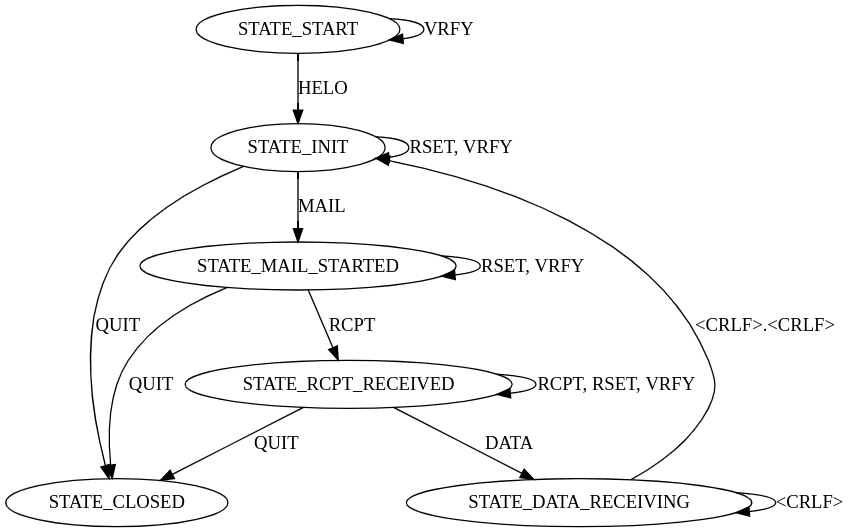
\includegraphics[scale=0.5]{smtp}
		\caption{Конечный автомат} 
	\end{figure}

	Были выделены следующие состояния конечного автомата:
	\begin{enumerate}
		\item init - данное состояние определяет, что клиент находится в невалидном для обмена данными состоянии, т.е. соединение с сервером не установлено, сокет не был открыт.
		\item connection - данное состояние определяет, что клиент успешно подключился к серверу, и может выполнять доступные ему команды, в данном случае SMTP-клиент может выполнить только 2 команды HELO и QUIT. Выполнение команды QUIT происходит только тогда, когда SMTP-сервер ответил клиенту сообщением с кодом отклика, означающего ошибку, тогда клиент инициирует закрытие сокета.
		\item start transaction - после выполнения команды HELO, когда клиент находится в состоянии connection,
		 он переходит в состояние start transaction, которое обозначает, что можно начинать выполнять
		  SMTP-транзакцию.
		   Подготовка к передаче данных осуществляется путем выполнения команды MAIL,
		    если сервер при ее выполнении возвращает сообщение с кодом отклика об успехе,
			 иначе на данном этапе клиент произведен завершение сессии путем перехода в состояние close с помощью команды QUIT.
		\item transaction - данное состояние определяет то, что MAIL прошел успешно и теперь
		 требуется отправить адреса получателей. 
		 Выполняется команда RCTP. При возникновении ошибок выполненяется команда QUIT.
		 В случае сообщения об отсутствии адреса электронного ящика на сервере клиент не прекратит 
		 попытки отправки по причине того, что другие электронные ящики могут присутствовать на сервер
		  и это сообщение будет доставлено кому-нибудь.
		   Переход из данного состояние в следующее производится при помощи выполнения команды
		    DATA, когда все адресаты переданы.
			 Если ни один из переданных адресов не был принят, сервер возвращает ошибку, 
			 которая приводит к инициированию закрытия соединения с помощью команды QUIT и переход в состояние close.
		\item sending data - данное состояние описывает процесс принятия данных сообщения. 
		 В случае каких-либо критических ошибок клиент инициирует закрытие соединения с помощью выполнения команды QUIT.
		  Переход в следующее состояние производится путем передачи флага завершения сообщения \textit{CRLF.CRLF},
		   данный флаг представлен на рисунке переходом в виде SEND END. 
		   В случае успешно переданного сообщения клиент переходит в состояние start transaction,
		    иначе будет иницировано закрытие соединения с помощью выполнения команды QUIT.
		\item close - данное состояние определяет, что соединение с сервером разорвано.
	\end{enumerate}

	\section{Описание формата хранения писем в файловой системе}
    	
	Для хранения текстов писем и дополнительной информации, которую принимает сервер во время SMTP-транзакции,
	 используется файловая система.
	
	\textbf{Maildir} - распространенный формат хранения электронной почты, 
	нетребующий монопольного захвата файла для обеспечения целостности почтового ящика при чтении, 
	добавлении или изменении сообщения. Каждое сообщение хранится в отдельном файле с уникальным именем, 
	а каждая папка представляет собой каталог. Вопросами блокировки файлов при добавлении, 
	перемещении и удалении файлов занимается локальная файловая система. 
	Все изменения делаются при помощи атомарных файловых операций, таким образом, монопольный захват файла 
	ни в каком случае не нужен.

	В случае стандартного \textit{Maildir} структура каталогов следующая:
	\begin{Verbatim}
	-home
		-user1
			-Maildir
				-cur
				-new
				-tmp
		-user2
			-Maildir
				-cur
				-new
				-tmp

	\end{Verbatim}

	В связи с некоторыми требованиями по использованию стандартного \textit{Maildir}, 
	таким как создание множества пользователей на устройстве, где запущен SMTP-сервер, 
	было решено модифицировать структуру \textit{Maildir} таким образом, 
	чтобы он содержал письма всех пользователей в едином каталоге.
	 Поскольку также \textit{Maildir} предназначен для доставки только локальной почты,
	  а по условию требуется пересылать также удаленную почту,
	   был добавлена новая директория для удаленной почты, 
	   где содержатся папки с почтой, предназначенной для удаленных SMTP-сервером. 
	   Структура каталогов модифицированного \textit{Maildir}:
        
    	\begin{verbatim}
        - maildir
               	-user1
                       	-cur
                       	-tmp
                       	-new
               	-user2
                       	-cur
                       	-tmp
                       	-new
               	.OTHER_SERVERS
                       	-server1
                               	-error
                               	-letter1
                               	-letter2
                       	-server2
                               	-error
                               	-letter3
                               	-letter4
    	\end{verbatim}

	\begin{itemize}
		\item maildir - корневой каталог \textit{Maildir}.
		\item user1, user2 - имена и каталоги пользователей SMTP-сервера, работающего на данном устройстве.
		\item cur - папка, содержащая прочитанную почту пользователем.
		\item tmp - папка, содержащая письма на стадии доставки, запись в файл не является атомарной операцией, 
		поэтому пока производится запись в файл отправка этих данных недопустима.
		\item new - папка, содержащая файлы писем, которые готовы к отправке.
		\item .OTHER\_SERVERS - каталог, содержащий папки с письмами для удаленных SMTP-серверов.
		\item server1, server2 - каталоги, содержащие письма для конкретных удаленных 
		сервером с доменным именем по имени данного каталога.
		\item letter1, letter2, letter3, letter4 - письма удаленной почты готовые для отправки, 
		содержатся сразу в каталогах, предназначенных для удаленных SMTP-серверов.
	\end{itemize}
    
	SMTP-клиенту как части MTA достаточно читать письма из каталога \textit{.OTHER\_SERVERS}, 
	а также удалять их из директории.
	

	\section{Взаимодействие клиента и сервера}

	В процессе курсовой работы требовалось разработать SMTP-клиент как часть MTA 
	для организации удаленной доставки письма после его получения и записи в каталог MAILDIR. 

	На рисунке 2.2 изображена диаграмма последовательности взяимодействия клиента с сервером
	\begin{figure}
		\centering
		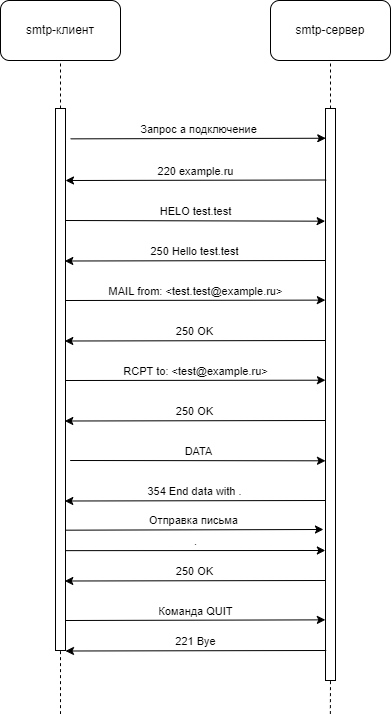
\includegraphics[scale = 2]{diagram.png}
		\caption{Диграмма последовательности взаимодействия клиента с сервером} 
	\end{figure}

	Организация удаленной доставки может быть обеспечена следующим образом:
	\begin{enumerate}
		\item Определение имени сервера по пути сервера, 
		в каталоге в MAILDIR которого находятся письма, 
		для определения того, куда необходимо передавать доступные для удаленной доставки письма.
		\item Открытие необходимого соединения SMTP-клиента c SMTP-сервером для последующей сессии.
		\item Начало сессии и инициирование общения с ним c помощью команды HELO.
		\item Считывание данных письма и последующий анализ дополнительных заголовков необходимых для последующей отправки.
		\item Передача адреса почтового ящика отправителя в MAIL. Данный адрес считывается из заголовков письма.
		\item Передачи всех возможных адресов получателей, которые были считаны из текста файла, содержащего текст письма.
		\item Передача команды DATA.
		\item Передача текста письма.
		\item Передача флага текста письма и получение сообщения.
		\item В случае успеха файл доставленного сообщение удаляется. 
		В случае неудачи, на каком-то из шагов сообщение перемещается в папку \/error.
		\item Если есть еще сообщения, то можем продолжить отправку, иначе закрыть соединение
		 и завершить сессию до появления новых сообщений.
	\end{enumerate}
	

	От SMTP-клиента требуется возможность подключения к нескольким удаленным SMTP-серверам.
	Требовалось разработать SMTP-клиент таким образом,
	 чтобы он обрабатывал несколько исходящих соединений в одном процессе. Требуется воспользоваться вызовом poll.

	 Системный вызов poll предоставляет пользователю механизм одновременного управления вводом/выводом (мультиплексирования) для набора дескрипторов открытых потоков. Для использования poll 
	 нужно инициализировать члены структуры pollfd наблюдаемыми дескрипторами и событиями, а затем вызвать poll().

	 Особенностями poll является:
	 \begin{itemize} 
		\item Отсутствие лимита количества наблюдаемых дескрипторов, можно мониторить более 1024 штук.
		\item Не модифицируется структура pollfd, что даёт возможность её переиспользования между вызовами poll()
	  — нужно лишь обнулить поле revents.
	\end{itemize}

	\chapter{Технологический раздел}


	\section{Описание процесса работы SMTP-клиента}

	Работа программы начинается с того, что запускается подсистема логгирования, 
	которая представляет собой отдельный процесс,который создаетя с помощью вызова \textit{fork()} и очереди сообщений.
	 В процессе выполнения процесса исполнения, предназначенного для логгирования, 
	 выполняется получение сообщения из очереди и сохранение его в файл.
	  Файл, в котором описаны все функции для работы с подсистемой логгирования, представлен в файле \textit{common/logs.c}.


	Далее производится загрузка конфигурации SMTP-клиента.
	 Конфигурация представляет из себя параметры
	   Полный путь до \textit{Maildir} настраивается с помощью параметра \textit{application.maildir.path}.
	    Конфигурация позволяет включать режим отладки с помощью параметра \textit{application.debug}, 
		который активирует (или деактивирует) печать логов типа \textit{DEBUG}. 
		Также конфигурация позволяет настраивать доменное имя текущего сервера с помощью параметра \textit{hostname}. 
		Чтение конфигурационного файла реализовано посредством бибилотеки \textit{libconfig}.

	Если загрузка конфигурации произошла с ошибкой,
	 то произойдет завершение работы программы путем освобождения ресурсов 
	 уже отданных под конфигурацию и остановка подсистемы логгирования.
		

	Далее вызывается функция  \textit{run\_client()}, описанная в файле \textit{client.c} .
	В начале работы этой функции производится инициализация основного контекста работы программы.
	Затем выполняется запус кается цикл \textit{while(1)}, в котором описана вся основная логика.
	
	Выполняется считывание дирректории \textit{Maildir} определяются новые удаленные серверы и новые письма для каждого сервера.
	Данная логика описана в файле.
	Если для определенного сервера есть письма выполняется открытие соединения с сервером. Для этого определяется MX-запись, и на полученный  ip-адрес на TCP-порт 25 выполняется подключение.
	Логика, для подключения описана в файле

	После успешного подключения к серверу его сокет добавляется в структуру \textit{pollfd}.
	
	Выполняется вызов \textit{poll()}, затем идет логика по определения текущего состояния, и принятия решения о следующей команде.

	Логика, реализующая конечный автомат,
	 находится так же в файле \textit{client.c}. 
	  Конечный автомат реализуется при помощи проверки состояния в блоке \textit{switch case}. 
	  Сама отправка SMTP-команд и письма реализуется в файле \textit{smtp.c}.

	  Для компилирования клиента и отчета используется утилита make. 
	  Фаил сборки представлен в листинге ниже
	  \begin{Verbatim}
CC = gcc
CFLAGS = -Wall -Werror -std=gnu99 -ggdb3
LFLAGS = -lrt -lconfig -D__GNU_SOURCE -lresolv

INCLUDES = -I include -I ../common/include 
CLIENT_SRC = main.c util.c ../common/log.c  config.c directory.c smtp.c client.c
OBJ_DIR = obj

OBJECTS = $(patsubst %.o,$(OBJ_DIR)/%.o, $(CLIENT_SRC:.c=.o))

all: client

client: $(CLIENT_SRC)
	$(CC) $(CFLAGS) $(CLIENT_SRC) $(INCLUDES) $(LFLAGS) -o client

clean:
	rm -rf *.o

	  \end{Verbatim}

	\chapter{Заключение}

	В результате выполнения данной курсовой работы был изучен протокол SMTP. 
	Разработан и реализован SMTP-клиент как часть MTA. 
	Был изучен системный вызов poll() для опроса набора сокетов. 
	 Разработка SMTP-клиента сопровождалась построением диаграмм,
	  в том числе и конечного автомата для последующей разработке 
	  общения SMTP-клиента с удаленным SMTP-сервером. 
	  Проведено ручное тестирование.
	
	В заключение можно сделать вывод, что все поставленные задачи в рамках курсовой работы по 
	разработке SMTP-клиента как части MTA были выполнены.


	\chapter{Список литературы}

	\begin{enumerate}
		\item rfc2821. Simple Mail Transfer Protocol [Электронный ресурс]. URL: http://rfc.com.ru/rfc2821.htm .
		\item Wikipedia.org. SMTP [Электронный ресурс]. URL: https://ru.wikipedia.org/wiki/SMTP .
		\item Хабр. select / poll / epoll: практическая разница [Электронный ресурс]. URL: https://habr.com/ru/company/infopulse/blog/415259/.
		\item Wikipedia.org. Maildir [Электронный ресурс]. URL: https://ru.wikipedia.org/wiki/Maildir
	\end{enumerate}
	
\end{document}
